\documentclass[12pt, a4paper]{report}

% Packages
\usepackage[utf8]{inputenc}
\usepackage[T1]{fontenc}
\usepackage[french]{babel}
\usepackage{mathptmx} % Times New Roman
\usepackage[left=2.5cm,right=2.5cm,top=2.5cm,bottom=2.5cm]{geometry}
\usepackage{setspace}
\usepackage{titlesec}
\usepackage{graphicx}
\usepackage{fancyhdr}
\usepackage{hyperref}
\usepackage{tikz}
\usetikzlibrary{shapes,arrows,positioning,shadows,calc}
\usepackage{float}
\usepackage{indentfirst}
\usepackage{caption}

% Configuration des paragraphes
\setlength{\parindent}{0.5cm}
\onehalfspacing

% Configuration des Titres
\titleformat{\chapter}[block]
  {\normalfont\fontsize{16}{19}\bfseries\centering}
  {\thechapter.}
  {1em}
  {}
\titlespacing*{\chapter}{0pt}{12pt}{12pt}

\titleformat{\section}
  {\normalfont\fontsize{14}{17}\bfseries}
  {\thesection.}
  {1em}
  {}
\titlespacing*{\section}{0pt}{12pt}{12pt}

\titleformat{\subsection}
  {\normalfont\fontsize{14}{17}\bfseries}
  {\thesubsection.}
  {1em}
  {}
\titlespacing*{\subsection}{0pt}{6pt}{12pt}

% En-têtes et Pieds de page Dynamiques
\pagestyle{fancy}
\fancyhf{}
\fancyhead[L]{\leftmark} 
\fancyhead[R]{\thepage}
\renewcommand{\chaptermark}[1]{\markboth{\thechapter.\ #1}{}}
\renewcommand{\headrulewidth}{0.4pt}

% Métadonnées PDF
\hypersetup{
    pdftitle={Rapport de Stage de Perfectionnement},
    pdfauthor={Étudiant},
    pdfsubject={Central de Réclamation}
}

\begin{document}

% Page de Garde
\begin{titlepage}
    \centering
    {\small Ministère de l’Enseignement Supérieur et de la recherche scientifique\\
    Direction Générale des Etudes Technologiques\\
    Institut Supérieur des Etudes Technologiques de Sfax\\
    Département Technologies de l’Informatique\par}
    
    \vspace{2cm}
    
    \begin{flushleft}
    Code stage : ........................\\
    Soutenu le : ........................
    \end{flushleft}
    
    \vspace{2cm}
    
    {\Huge \textbf{STAGE DE PERFECTIONNEMENT}\par}
    
    \vspace{2cm}
    
    \begin{minipage}{0.45\textwidth}
        \textbf{Organisme d’accueil :}\\[0.5cm]
        \textbf{SCPC Comptoir Hammami}
    \end{minipage}
    \hfill
    \begin{minipage}{0.45\textwidth}
        \textbf{Elaboré par :}\\[0.5cm]
        \textbf{FRIKHA Mariem}
    \end{minipage}
    
    \vfill
    
    {\large Année Universitaire : 2025/2026\par}
\end{titlepage}

% Sommaire
\tableofcontents
\newpage

% Liste des figures et tableaux (Ajout pour volume)
\listoffigures
\addcontentsline{toc}{chapter}{Liste des figures}
\newpage

\listoftables
\addcontentsline{toc}{chapter}{Liste des tableaux}
\newpage

% --- CONTENU MODULAIRE ---

\chapter*{Remerciements}
\addcontentsline{toc}{chapter}{Remerciements}

Je tiens à remercier vivement mon encadreur de stage au sein de la société SCPC Comptoir Hammami pour son accueil, sa disponibilité et ses précieux conseils tout au long de cette période.

Mes remerciements s'adressent également à tout le personnel de l'entreprise pour leur collaboration et l'environnement de travail agréable qu'ils ont su créer.

Enfin, je remercie mes enseignants de l'ISET de Sfax pour la qualité de la formation dispensée, qui m'a permis de mener à bien ce projet.

\newpage

\chapter*{Introduction}
\addcontentsline{toc}{chapter}{Introduction}

Le stage de perfectionnement représente une étape cruciale dans la formation de l'étudiant, lui permettant de confronter ses acquis théoriques aux réalités du monde professionnel. C'est dans ce cadre que j'ai eu l'opportunité d'effectuer mon stage au sein de la société SCPC Comptoir Hammami.

L'objectif de ce stage était de concevoir et développer une application web, intitulée "Central de Réclamation", destinée à moderniser et optimiser la gestion des réclamations clients, qui était jusqu'alors traitée manuellement.

Ce rapport retrace les différentes étapes de ce projet, de l'étude de l'existant à la réalisation finale. Il est structuré comme suit :
\begin{itemize}
    \item \textbf{Chapitre 1 : Etude de l'organisme.} Présentation de la société SCPC Comptoir Hammami et de son environnement.
    \item \textbf{Chapitre 2 : Présentation du thème.} Définition du périmètre du projet et planning prévisionnel.
    \item \textbf{Chapitre 3 : Infrastructure informatique.} Description des ressources matérielles et logicielles.
    \item \textbf{Chapitre 4 : Etude préalable.} Analyse de l'existant, critique et justification de la solution.
    \item \textbf{Chapitre 5 : Etude conceptuelle.} Conception UML (Cas d'utilisation, Séquence, Classes).
    \item \textbf{Chapitre 6 : Réalisation.} Présentation de l'architecture, de la sécurité et des interfaces finales.
\end{itemize}

\newpage

\chapter{Étude de l'organisme}

\section*{Introduction}
Ce premier chapitre a pour vocation de présenter le cadre général dans lequel s'est déroulé ce stage. Il offre une vue d'ensemble sur le Groupe Hammami, son historique et son poids économique, avant de se focaliser sur la société d'accueil, la SCPC Comptoir Hammami, et son organisation interne. Cette présentation permet de mieux appréhender le contexte professionnel et les enjeux industriels de l'entreprise.

\section{Présentation du Groupe Hammami}
Le Groupe Hammami est un acteur majeur du secteur du Bâtiment et des Travaux Publics (BTP) en Tunisie. Créé grâce à la vision et à l'engagement de feu Mahmoud Hammami, il s'est développé pour inclure 18 sociétés, opérant dans divers domaines du BTP. Le flambeau a été repris par ses fils, Messieurs Habib, Khaled, Hafedh et Khalil, qui perpétuent la mission d'excellence et d'innovation du groupe.

Avec une présence nationale et une portée internationale, le Groupe Hammami exporte ses produits vers plusieurs pays africains, notamment la Libye, le Maroc, le Sénégal, le Ghana et bien d'autres. En collaborant avec des partenaires tunisiens et étrangers, le groupe aspire à offrir des solutions adaptées aux besoins des marchés modernes.

\begin{itemize}
    \item \textbf{Secteur d’activité :} Commerce et développement international.
    \item \textbf{Taille de l’entreprise :} Entre 1 001 et 5 000 employés.
    \item \textbf{Siège social :} Sfax et Tunis, Tunisie.
\end{itemize}

\begin{figure}[H]
    \centering
    % \includegraphics[width=0.5\textwidth]{assets/images/logo_groupe_hammami.png}
    \caption{logo du Groupe Hammami}
    \label{fig:logo_groupe}
\end{figure}

\begin{figure}[H]
    \centering
    % \includegraphics[width=0.8\textwidth]{assets/images/societes_groupe.png}
    \caption{Sociétés du groupe Hammami}
    \label{fig:societes_groupe}
\end{figure}

\section{Présentation de la SCPC Comptoir Hammami}
Créée en 1999, la SCPC Comptoir Hammami est une filiale du Groupe Hammami, spécialisée dans le commerce en gros des matériaux de construction. Elle offre une gamme complète de solutions adaptées aux besoins du secteur BTP, allant des matériaux pour le gros œuvre aux équipements de chantier et aux systèmes de revêtement.

L’entreprise collabore avec les plus grands producteurs européens pour garantir des produits répondant aux standards de qualité, sécurité et compétitivité. Grâce à son service logistique, elle assure des livraisons sur l’ensemble du territoire tunisien.

\begin{itemize}
    \item \textbf{Secteur d’activité :} Commerce de gros.
    \item \textbf{Taille de l’entreprise :} Entre 51 et 200 employés.
    \item \textbf{Siège social :} Sfax, Tunisie.
    \item \textbf{Certifications :} ISO 9001:2015.
\end{itemize}

\begin{figure}[H]
    \centering
    % \includegraphics[width=0.5\textwidth]{assets/images/logo_scpc.png}
    \caption{Logo comptoir Hammami}
    \label{fig:logo_scpc}
\end{figure}

\subsection{Produits}
La SCPC Comptoir Hammami propose une large gamme de produits couvrant les besoins du BTP. Les principales catégories incluent :
\begin{itemize}
    \item \textbf{Gros œuvre :} Ciment, fer à béton, treillis soudés, colle de bâtiment, chimie de bâtiment.
    \item \textbf{Bois et panneaux :} Bois de coffrage, contreplaqués, systèmes de coffrage.
    \item \textbf{Isolation et étanchéité :} Solutions pour isolation thermique et acoustique.
    \item \textbf{Matériel BTP :} Bétonnières, groupes électrogènes, convertisseurs, talocheuses.
    \item \textbf{Revêtements et décoration :} Carrelages, tuiles, bordures et pavés.
\end{itemize}

\subsection{Activités principales}
Les activités de la SCPC Comptoir Hammami s’articulent autour des processus suivants :
\begin{itemize}
    \item \textbf{Commercial :} Gestion des ventes, promotion, relation client.
    \item \textbf{Finance et comptabilité :} Gestion de trésorerie, rapprochements bancaires, comptabilité générale et analytique.
    \item \textbf{Ressources humaines :} Formation, rémunération, gestion administrative du personnel.
    \item \textbf{Informatique :} Maintenance des équipements, gestion réseau, ERP et sécurité informatique.
\end{itemize}

\subsection{Organigramme de la société}
La SCPC Comptoir Hammami est structurée pour maximiser son efficacité opérationnelle. Un organigramme clair définit les rôles et responsabilités des différents départements, incluant des équipes dédiées à la gestion informatique, à la logistique, et aux services commerciaux.

\begin{figure}[H]
    \centering
    % \includegraphics[width=0.8\textwidth]{assets/images/organigramme.png}
    \caption{Organigramme de la société}
    \label{fig:organigramme}
\end{figure}

\section*{Conclusion}
Ce chapitre nous a permis de situer le stage dans son contexte organisationnel. La compréhension de la structure du Groupe Hammami et du fonctionnement de la SCPC est essentielle pour saisir les enjeux du projet. C'est au sein de cet environnement dynamique que s'inscrit la mission présentée dans le chapitre suivant.

\newpage

\chapter{Contexte général et étude préalable}

\section*{Introduction}
La réussite d'un projet informatique dépend d'une compréhension profonde de son environnement et des besoins réels de ses utilisateurs. Ce chapitre pose les fondations de notre travail en présentant d'abord le cadre du projet, la problématique rencontrée et les objectifs visés. Nous détaillerons ensuite l'étude de l'existant afin de justifier les choix de conception qui ont guidé le développement de la solution "Central de Réclamation".

\section{Présentation du thème du stage}
Le stage effectué au sein de la société SCPC Comptoir Hammami s'inscrit dans une optique de modernisation des processus internes. Face à l'accroissement du volume d'activités et à l'exigence croissante en matière de qualité de service, il est devenu impératif de repenser la gestion des réclamations clients.

\subsection{Problématique}
Actuellement, la gestion des réclamations au sein de la SCPC repose sur des processus qui peuvent manquer de fluidité ou de traçabilité centralisée. Les informations circulent entre différents services (Commercial, Qualité, Fournisseur) parfois via des canaux dispersés (téléphone, emails non structurés), ce qui peut entraîner :
\begin{itemize}
    \item Une perte d'information ou des délais de réponse allongés.
    \item Une difficulté à obtenir une vision globale des statistiques de non-conformité.
    \item Un manque de visibilité pour le client sur l'avancement de son dossier.
\end{itemize}

\subsection{Objectifs du projet}
Les principaux objectifs assignés à ce stage sont :
\begin{enumerate}
    \item Analyser les besoins fonctionnels des différents acteurs.
    \item Concevoir une architecture logicielle robuste et évolutive.
    \item Développer l'application en utilisant des technologies web standards.
    \item Garantir la fiabilité des données et la sécurité des accès.
\end{enumerate}

\section{Étude de l'existant}
L'étude préalable permet de comprendre le fonctionnement actuel de l'organisme et de déceler les failles nécessitant une intervention informatique.

\subsection{Description du processus actuel}
Avant le démarrage du projet, le flux de traitement des réclamations se caractérisait par l'absence d'outils dédiés :
\begin{itemize}
    \item \textbf{Saisie Manuelle :} Les informations sont notées sur papier ou envoyées par email non structuré.
    \item \textbf{Centralisation sur Excel :} Le Responsable Qualité (RMQ) doit ressaisir manuellement les données dans un fichier Excel local ("Registre des Non-Conformités").
    \item \textbf{Suivi Opaque :} Pour connaître l'état d'un dossier, le client ou le commercial doit appeler manuellement le service qualité.
\end{itemize}

\subsection{Critiques de l'existant}
Ce fonctionnement présente des limites majeures :
\begin{itemize}
    \item \textbf{Limites Organisationnelles :} Absence de traçabilité, perte de temps liée à la ressaisie, manque de réactivité.
    \item \textbf{Limites Techniques :} Risque de perte de données (Excel unique/local), absence de statistiques automatisées, impossibilité de travail collaboratif fluide.
\end{itemize}

\section{Solution proposée : "Central de Réclamation"}
Face à ces constats, le développement d'une application web sur mesure a été retenu. Cette solution informatique vise à dématérialiser l'intégralité du flux de traitement :
\begin{itemize}
    \item \textbf{Développement spécifique :} Coller parfaitement au workflow de validation qualité de la SCPC.
    \item \textbf{Centralisation :} Une base de données unique accessible en temps réel par tous les acteurs (Clients, Commerciaux, RMQ, AQF).
    \item \textbf{Automatisation :} Notification automatique par email et calcul instantané des indicateurs de performance.
\end{itemize}

\section*{Conclusion}
Ce chapitre a permis de fusionner le cadre du stage et l'analyse de l'existant, mettant en évidence la nécessité de moderniser le système de gestion des réclamations. Le passage d'une gestion manuelle sur Excel à une plateforme interactive constitue le socle du projet. Le chapitre suivant présentera l'infrastructure technique nécessaire à la réalisation de cette solution.

\newpage

\chapter{Environnement de travail et ressources technologiques}

\section*{Introduction}
La réalisation d'un projet informatique nécessite un environnement de travail adéquat, composé de ressources matérielles performantes et d'outils logiciels adaptés. Ce chapitre détaille l'infrastructure technique utilisée durant la période de stage pour mener à bien les phases de conception, développement et rédaction.

\section{Environnement Matériel}
Pour le développement de l'application et la rédaction du rapport, j'ai utilisé un ordinateur portable personnel dont les caractéristiques garantissent une fluidité d'exécution des différents outils.

\textbf{Caractéristiques de l'ordinateur de développement :}
\begin{itemize}
    \item \textbf{Processeur :} Processeurs multicœurs (Intel i7/AMD Ryzen 7 ou équivalents) pour une exécution rapide des compilations et des tests.
    \item \textbf{Mémoire RAM :} 16 Go de RAM pour assurer une fluidité lors de l'exécution simultanée des serveurs locaux, des IDE, et des navigateurs pour le test.
    \item \textbf{Stockage :} Disque SSD (1 To ou plus) pour un accès rapide aux fichiers et aux données.
\end{itemize}

\section{Environnement Logiciel}
Dans cette partie, nous allons présenter les différents outils informatiques utilisés pour le développement, la modélisation et le déploiement.

\subsection{Développement et Tests Locaux}

\noindent
\begin{minipage}[c]{0.3\textwidth}
    \centering
    
\includegraphics[width=0.6\textwidth]{images/vscode.png}
    \captionof{figure}{Visual Studio Code}
\end{minipage}
\hfill
\begin{minipage}[c]{0.65\textwidth}
    \textbf{Visual Studio Code (VS Code) :} L'éditeur de code principal utilisé pour ce projet. Sa polyvalence et ses extensions (PHP IntelliSense, GitLink) en font un outil incontournable.
\end{minipage}

\vspace{0.6cm}

\noindent
\begin{minipage}[c]{0.3\textwidth}
    \centering
    
\includegraphics[width=0.6\textwidth]{images/xampp.png}
    \captionof{figure}{XAMPP}
\end{minipage}
\hfill
\begin{minipage}[c]{0.65\textwidth}
    \textbf{XAMPP :} Utilisé comme environnement de serveur local (Apache + MySQL + PHP) pour tester l'application avant son déploiement.
\end{minipage}

\vspace{0.6cm}

\subsection{Langages et Technologies Web}

\noindent
\begin{minipage}[c]{0.3\textwidth}
    \centering
    
\includegraphics[width=0.5\textwidth]{images/html.png}
    \captionof{figure}{HTML5}
\end{minipage}
\hfill
\begin{minipage}[c]{0.65\textwidth}
    \textbf{HTML5 :} Langage de balisage utilisé pour la structuration sémantique et le contenu des pages web. Il constitue le squelette de l'application.
\end{minipage}

\vspace{0.6cm}

\noindent
\begin{minipage}[c]{0.3\textwidth}
    \centering
    
\includegraphics[width=0.5\textwidth]{images/css.png}
    \captionof{figure}{CSS3}
\end{minipage}
\hfill
\begin{minipage}[c]{0.65\textwidth}
    \textbf{CSS3 :} Langage de feuilles de style utilisé pour la mise en forme graphique, le design responsive et l'esthétique globale de l'interface utilisateur.
\end{minipage}

\vspace{0.6cm}

\noindent
\begin{minipage}[c]{0.3\textwidth}
    \centering
    
\includegraphics[width=0.5\textwidth]{images/php.png}
    \captionof{figure}{PHP}
\end{minipage}
\hfill
\begin{minipage}[c]{0.65\textwidth}
    \textbf{PHP :} Langage de script côté serveur, utilisé pour le développement de la logique métier, la gestion des sessions utilisateurs et les interactions avec la base de données. Il constitue le moteur dynamique de l'application.
\end{minipage}

\vspace{0.6cm}

\noindent
\begin{minipage}[c]{0.3\textwidth}
    \centering
    
\includegraphics[width=0.5\textwidth]{images/js.png}
    \captionof{figure}{JavaScript}
\end{minipage}
\hfill
\begin{minipage}[c]{0.65\textwidth}
    \textbf{JavaScript :} Langage de programmation côté client permettant d'enrichir l'expérience utilisateur via des interactions dynamiques, la validation de formulaires en temps réel et la gestion des menus interactifs.
\end{minipage}

\vspace{0.6cm}

\subsection{Système de Gestion de Base de Données}

\noindent
\begin{minipage}[c]{0.3\textwidth}
    \centering
    
\includegraphics[width=0.6\textwidth]{images/mysql.png.jpg}
    \captionof{figure}{MySQL}
\end{minipage}
\hfill
\begin{minipage}[c]{0.65\textwidth}
    \textbf{MySQL :} Système de gestion de base de données relationnelle (SGBDR) robuste et performant. Il assure le stockage structuré, la persistance et l'intégrité des données du système d'information.
\end{minipage}

\vspace{0.6cm}

\subsection{Bibliothèques et Outils Tiers}

\noindent
\begin{minipage}[c]{0.3\textwidth}
    \centering
    
\includegraphics[width=0.5\textwidth]{images/bootstrap.png}
    \captionof{figure}{Bootstrap}
\end{minipage}
\hfill
\begin{minipage}[c]{0.65\textwidth}
    \textbf{Bootstrap :} Framework CSS populaire utilisé pour accélérer le développement front-end et garantir une interface parfaitement responsive, s'adaptant à tous les types d'écrans (mobiles, tablettes, desktop).
\end{minipage}

\vspace{0.6cm}

\noindent
\begin{minipage}[c]{0.3\textwidth}
    \centering
    
\includegraphics[width=0.5\textwidth]{images/fontawesome.png}
    \captionof{figure}{Font Awesome}
\end{minipage}
\hfill
\begin{minipage}[c]{0.65\textwidth}
    \textbf{Font Awesome :} Bibliothèque d'icônes vectorielles offrant une large gamme de symboles graphiques pour améliorer la lisibilité et l'ergonomie des interfaces utilisateurs.
\end{minipage}

\vspace{0.6cm}

\noindent
\begin{minipage}[c]{0.3\textwidth}
    \centering
    
\includegraphics[width=0.6\textwidth]{images/phpmailer.png}
    \captionof{figure}{PHPMailer}
\end{minipage}
\hfill
\begin{minipage}[c]{0.65\textwidth}
    \textbf{PHPMailer :} Bibliothèque PHP complète et sécurisée pour la gestion de l'envoi d'emails. Elle est utilisée pour les notifications automatiques et l'envoi de confirmations aux utilisateurs.
\end{minipage}

\subsection{Déploiement et Hébergement}

\noindent
\begin{minipage}[c]{0.3\textwidth}
    \centering
    \includegraphics[width=0.6\textwidth]{images/ovh.jpg}
    \captionof{figure}{OVHcloud}
\end{minipage}
\hfill
\begin{minipage}[c]{0.65\textwidth}
    \textbf{OVHcloud :} Fournisseur d'hébergement choisi pour la mise en ligne de l'application. Sa fiabilité et ses serveurs sécurisés garantissent la disponibilité de la plateforme.
\end{minipage}

\section*{Conclusion}
Ce chapitre a permis de dresser le panorama technique du projet. De l'environnement matériel robuste à la suite logicielle intégrant des technologies web fondamentales (HTML, CSS, JavaScript et MySQL), l'infrastructure a été pensée pour allier performance, sécurité et maintenabilité.

\newpage

\chapter{Étude conceptuelle}

\section*{Introduction}
Après avoir cerné les besoins et les contraintes du projet dans l'étude préalable, il est essentiel de passer à la phase de conception. Ce chapitre se consacre à la modélisation détaillée du système "Central de Réclamation". En s'appuyant sur le langage UML (Unified Modeling Language), nous allons définir l'architecture statique et dynamique de l'application, garantissant ainsi une base solide pour le développement futur.

\section{Diagramme de Cas d'Utilisation Global}
Le diagramme suivant présente une vue d'ensemble exhaustive des interactions entre les différents acteurs et le système. Il met en évidence la séparation des responsabilités entre les clients, les commerciaux, le service qualité (RMQ/AQF) et l'administration. Les dépendances de type <<include>> et <<extend>> sont utilisées pour modéliser les fonctionnalités complexes telles que l'ajout de pièces jointes ou la notification automatique.

\begin{figure}[H]
    \centering
    \begin{tikzpicture}[scale=0.75, transform shape]
        % Système
        \draw[thick, fill=blue!2, rounded corners] (2.5,-12) rectangle (12,1);
        \node[font=\bfseries] at (7.25,1.4) {Système Central de Réclamation};
        
        % Acteurs (Généralisés)
        \node (client) at (0,0) [draw, circle, fill=green!10] {}; \node[below=0.1cm] at (client) {Client};
        \node (comm) at (0,-3) [draw, circle, fill=orange!10] {}; \node[below=0.1cm] at (comm) {Commercial};
        \node (rmq) at (0,-6) [draw, circle, fill=purple!10] {}; \node[below=0.1cm] at (rmq) {RMQ};
        \node (aqf) at (0,-9) [draw, circle, fill=teal!10] {}; \node[below=0.1cm] at (aqf) {AQF};
        \node (admin) at (14,-5) [draw, circle, fill=red!10] {}; \node[below=0.1cm] at (admin) {Admin};

        % Cas d'utilisation groupés par zone
        \node[draw, ellipse, fill=white, minimum width=3cm] (auth) at (7,0) {S'authentifier};
        \node[draw, ellipse, fill=white, minimum width=3.5cm] (creer) at (5.5,-2) {Créer réclamation};
        \node[draw, ellipse, fill=white, minimum width=3cm] (suivi) at (5.5,-3.5) {Suivre état};
        
        \node[draw, ellipse, fill=white, minimum width=3.5cm] (vrmq) at (9,-5) {Valider/Refuser};
        \node[draw, ellipse, fill=white, minimum width=3cm] (assign) at (9,-7) {Assigner AQF};
        
        \node[draw, ellipse, fill=white, minimum width=3.5cm] (traite) at (7,-9.5) {Traiter réclamation};
        \node[draw, ellipse, fill=white, minimum width=3.5cm] (stats) at (7,-11) {Consulter Stats};

        \node[draw, ellipse, fill=white, minimum width=3.5cm] (users) at (11.5,-4) {Gérer Utilisateurs};
        \node[draw, ellipse, fill=white, minimum width=3.5cm] (adminall) at (11.5,-6) {Vue globale};

        % Relations
        \draw (client) -- (auth); \draw (client) -- (creer); \draw (client) -- (suivi);
        \draw (comm) -- (auth); \draw (comm) -- (creer);
        \draw (rmq) -- (auth); \draw (rmq) -- (vrmq); \draw (rmq) -- (assign);
        \draw (aqf) -- (auth); \draw (aqf) -- (traite);
        \draw (admin) -- (auth); \draw (admin) -- (users); \draw (admin) -- (adminall);
        
        \draw (creer) -- (comm);
        \draw (rmq) -- (stats); \draw (aqf) -- (stats);
    \end{tikzpicture}
    \caption{Diagramme de Cas d'Utilisation Global}
    \label{fig:dcu_global}
\end{figure}

\section{Diagrammes de Séquence}
Les diagrammes de séquence illustrent les interactions temporelles entre les acteurs et le système pour des scénarios clés.

\subsection{Séquence : Acteur Client}
Le flux suivant montre comment une réclamation est traitée lors de sa création par le client. Il illustre l'interaction avec le contrôleur de tickets et le service de messagerie pour garantir que le client reçoit une confirmation immédiate de son dépôt.

\begin{figure}[H]
    \centering
    \begin{tikzpicture}[scale=0.85, transform shape]
        \node[draw, rectangle, fill=green!10] (cl) at (0,0) {Client};
        \node[draw, rectangle, fill=blue!10] (ctrl) at (4,0) {Contrôleur};
        \node[draw, rectangle, fill=orange!10] (mail) at (8,0) {EmailService};
        \draw[dashed] (cl) -- (0,-5); \draw[dashed] (ctrl) -- (4,-5); \draw[dashed] (mail) -- (8,-5);
        \draw[->] (0,-1) -- node[above, font=\scriptsize] {soumettreReclamation()} (4,-1);
        \draw[->] (4,-2) -- node[above, font=\scriptsize] {notifierClient()} (8,-2);
        \draw[<--] (0,-4) -- node[above, font=\scriptsize] {Confirmation (N° Ticket)} (4,-4);
    \end{tikzpicture}
    \caption{Diagramme de Séquence -- Création Client}
\end{figure}

\subsection{Séquence : Acteur Commercial}
Ce diagramme met en évidence le rôle de soutien du commercial. Il illustre la phase de recherche dans le référentiel client et le pré-remplissage dynamique du formulaire, permettant un gain de temps considérable lors des visites sur site.

\begin{figure}[H]
    \centering
    \begin{tikzpicture}[scale=0.85, transform shape]
        \node[draw, rectangle, fill=orange!10] (cm) at (0,0) {Commercial};
        \node[draw, rectangle, fill=blue!10] (ctrl) at (5,0) {TicketController};
        \draw[dashed] (cm) -- (0,-5); \draw[dashed] (ctrl) -- (5,-5);
        \draw[->] (0,-1) -- node[above, font=\scriptsize] {rechercherClient(code)} (5,-1);
        \draw[<--] (0,-2.5) -- node[above, font=\scriptsize] {infosProfil} (5,-2.5);
        \draw[->] (0,-4) -- node[above, font=\scriptsize] {creerCompteClient()} (5,-4);
    \end{tikzpicture}
    \caption{Diagramme de Séquence -- Aide Commerciale}
\end{figure}

\subsection{Séquence : Acteur RMQ}
Le Responsable Qualité intervient comme le pivot décisionnel. Le diagramme de séquence décrit ici le processus de validation d'une plainte, l'assignation d'un expert AQF et la mise à jour immédiate du statut, assurant la traçabilité de chaque action.

\begin{figure}[H]
    \centering
    \begin{tikzpicture}[scale=0.85, transform shape]
        \node[draw, rectangle, fill=purple!10] (rmq) at (0,0) {RMQ};
        \node[draw, rectangle, fill=blue!10] (ctrl) at (4,0) {WorkflowController};
        \node[draw, rectangle, fill=teal!10] (aqf) at (8,0) {AQF};
        \draw[dashed] (rmq) -- (0,-5); \draw[dashed] (ctrl) -- (4,-5); \draw[dashed] (aqf) -- (8,-5);
        \draw[->] (0,-1) -- node[above, font=\scriptsize] {validerTicket()} (4,-1);
        \draw[->] (4,-2.5) -- node[above, font=\scriptsize] {assigner(aqf\_id)} (8,-2.5);
        \draw[<--] (0,-4) -- node[above, font=\scriptsize] {Statut mis à jour} (4,-4);
    \end{tikzpicture}
    \caption{Diagramme de Séquence -- Validation RMQ}
\end{figure}

\subsection{Séquence : Acteur AQF}
Le diagramme suivant détaille la phase finale de résolution. L'expert AQF interagit avec le système pour consigner les décisions prises, joindre les preuves techniques et clôturer définitivement le dossier afin de libérer les ressources.

\begin{figure}[H]
    \centering
    \begin{tikzpicture}[scale=0.85, transform shape]
        \node[draw, rectangle, fill=teal!10] (aqf) at (0,0) {AQF};
        \node[draw, rectangle, fill=blue!10] (ctrl) at (5,0) {TraitementController};
        \draw[dashed] (aqf) -- (0,-5); \draw[dashed] (ctrl) -- (5,-5);
        \draw[->] (0,-1) -- node[above, font=\scriptsize] {ajouterSolution()} (5,-1);
        \draw[->] (0,-2.5) -- node[above, font=\scriptsize] {joindrePreuve(file)} (5,-2.5);
        \draw[->] (0,-4) -- node[above, font=\scriptsize] {clôturerTicket()} (5,-4);
    \end{tikzpicture}
    \caption{Diagramme de Séquence -- Résolution AQF}
\end{figure}

\subsection{Séquence : Administrateur}
Le rôle d'administration garantit l'intégrité du système. Ce flux montre la gestion du cycle de vie des utilisateurs, de la création de compte à la définition des droits d'accès, ainsi que la consultation des archives multi-annuelles.

\begin{figure}[H]
    \centering
    \begin{tikzpicture}[scale=0.85, transform shape]
        \node[draw, rectangle, fill=red!10] (adm) at (0,0) {Admin};
        \node[draw, rectangle, fill=blue!10] (ctrl) at (5,0) {AdminController};
        \draw[dashed] (adm) -- (0,-4); \draw[dashed] (ctrl) -- (5,-4);
        \draw[->] (0,-1.5) -- node[above, font=\scriptsize] {createUserAccount()} (5,-1.5);
        \draw[->] (0,-3) -- node[above, font=\scriptsize] {accessYearData(2025)} (5,-3);
    \end{tikzpicture}
    \caption{Diagramme de Séquence -- Maintenance Admin}
\end{figure}

\section{Diagramme de Classes Unique}
Le modèle statique présenté ci-après définit la structure de données du "Central de Réclamation". Il montre l'héritage entre l'entité Utilisateur et ses sous-classes, ainsi que la composition forte entre un Ticket et ses composants (Historique, Pièces Jointes, Commentaires).

\begin{figure}[H]
    \centering
    \begin{tikzpicture}[scale=0.6, transform shape]
        \tikzstyle{class}=[rectangle, draw, fill=white, minimum width=3cm, minimum height=1.5cm, text centered]
        \node[class] (user) at (0,0) {\textbf{Utilisateur}};
        \node[class] (ticket) at (6,0) {\textbf{Ticket}};
        \node[class] (client) at (-2,-3) {\textbf{Client}};
        \node[class] (personnel) at (2,-3) {\textbf{Personnel}};
        \node[class] (pj) at (6,-3) {\textbf{PieceJointe}};
        \node[class] (comm) at (10,-1.5) {\textbf{Commentaire}};
        
        \draw[->, thick] (user) -- (ticket);
        \draw[->] (client) -- (user); \draw[->] (personnel) -- (user);
        \draw[*-] (ticket) -- (pj); \draw[*-] (ticket) -- (comm);
    \end{tikzpicture}
    \caption{Diagramme de Classes du Système}
    \label{fig:diag-classes}
\end{figure}

\section*{Conclusion}
L'étude conceptuelle nous a permis de structurer la solution informatique dans ses moindres détails. Les diagrammes UML élaborés assurent une vision claire des interactions, des données et des processus. Cette étape de modélisation constitue le socle indispensable pour aborder sereinement la phase de développement et de réalisation.

\newpage

\chapter{Réalisation}

\section*{Introduction}
La phase de réalisation concrétise l'ensemble des études préalables et conceptuelles effectuées. Ce chapitre présente les aspects techniques de la mise en œuvre du système "Central de Réclamation", depuis la configuration de l'environnement de développement jusqu'à la présentation des interfaces utilisateurs finales, en passant par l'architecture logicielle retenue.

\section{Environnement de réalisation}
Pour concrétiser ce projet, nous avons mis en place un environnement de développement complet.

\subsection{Outils logiciels}
\begin{itemize}
    \item \textbf{Visual Studio Code :} Notre environnement de développement intégré (IDE) principal.
    \item \textbf{XAMPP :} Pour simuler un serveur de production en local (Apache/MySQL/PHP).
    \item \textbf{Git :} Pour le versionnage du code source.
    \item \textbf{PHPMailer :} Bibliothèque d'envoi d'emails SMTP.
\end{itemize}

\section{Architecture de l'application}
L'application repose sur une architecture MVC (Modèle-Vue-Contrôleur) simplifiée :
\begin{itemize}
    \item \textbf{Modèle :} Gestion des données (fichiers dans \texttt{/api/} et \texttt{/config/}).
    \item \textbf{Vue :} Interfaces utilisateurs (fichiers dans \texttt{/pages/}).
    \item \textbf{Contrôleur :} Logique métier et routage (fichier \texttt{index.php}).
\end{itemize}

\section{Interfaces Graphiques}
L'ergonomie a été travaillée pour offrir une expérience utilisateur fluide et professionnelle. Nous présentons ci-dessous les principales interfaces du système, organisées par espace utilisateur.

% ==================================================
% ESPACE CLIENT
% ==================================================
\subsection{Espace Client}

\subsubsection{Page d'Accueil et Authentification}
La page d'accueil permet aux utilisateurs (Clients et Personnel) de se connecter de manière sécurisée. Le design est épuré, aux couleurs de l'entreprise (Bleu et Blanc).

\begin{figure}[H]
    \centering
    
\includegraphics[width=14cm]{images/accueil_client.png}
    \caption{Interface d'accueil -- Page principale du système}
    \label{fig:accueil}
\end{figure}

\subsubsection{Formulaire de Nouvelle Réclamation}
Le formulaire de soumission permet au client de saisir les informations détaillées de sa réclamation, incluant la possibilité d'ajouter plusieurs produits et des pièces jointes.

\begin{figure}[H]
    \centering
    \fbox{\parbox{12cm}{\centering\vspace{3cm}\textit{Capture d'écran à insérer}\\[0.5cm]\texttt{images/form_nouvelle_reclamation.png}\vspace{3cm}}}
    \caption{Formulaire de création d'une nouvelle réclamation}
    \label{fig:form-reclamation}
\end{figure}

\subsubsection{Tableau de Bord Client}
Le dashboard client offre une vue centralisée de toutes les réclamations soumises avec leur statut actuel.

\begin{figure}[H]
    \centering
    \fbox{\parbox{12cm}{\centering\vspace{3cm}\textit{Capture d'écran à insérer}\\[0.5cm]\texttt{images/dashboard_client.png}\vspace{3cm}}}
    \caption{Tableau de bord de l'espace client}
    \label{fig:dashboard-client}
\end{figure}

% ==================================================
% ESPACE COMMERCIAL
% ==================================================
\subsection{Espace Commercial}

\subsubsection{Tableau de Bord Commercial}
L'interface commerciale permet aux agents de créer des réclamations au nom des clients et de suivre l'ensemble des tickets.

\begin{figure}[H]
    \centering
    \fbox{\parbox{12cm}{\centering\vspace{3cm}\textit{Capture d'écran à insérer}\\[0.5cm]\texttt{images/dashboard_commercial.png}\vspace{3cm}}}
    \caption{Tableau de bord de l'espace commercial}
    \label{fig:dashboard-commercial}
\end{figure}

% ==================================================
% ESPACE RMQ
% ==================================================
\subsection{Espace Responsable Management Qualité (RMQ)}

\subsubsection{Tableau de Bord RMQ}
Le tableau de bord RMQ permet une supervision globale des réclamations. Il affiche :
\begin{itemize}
    \item Des indicateurs statistiques en temps réel (KPI).
    \item La répartition des tickets par statut.
    \item La liste des derniers tickets reçus avec actions rapides.
\end{itemize}

\begin{figure}[H]
    \centering
    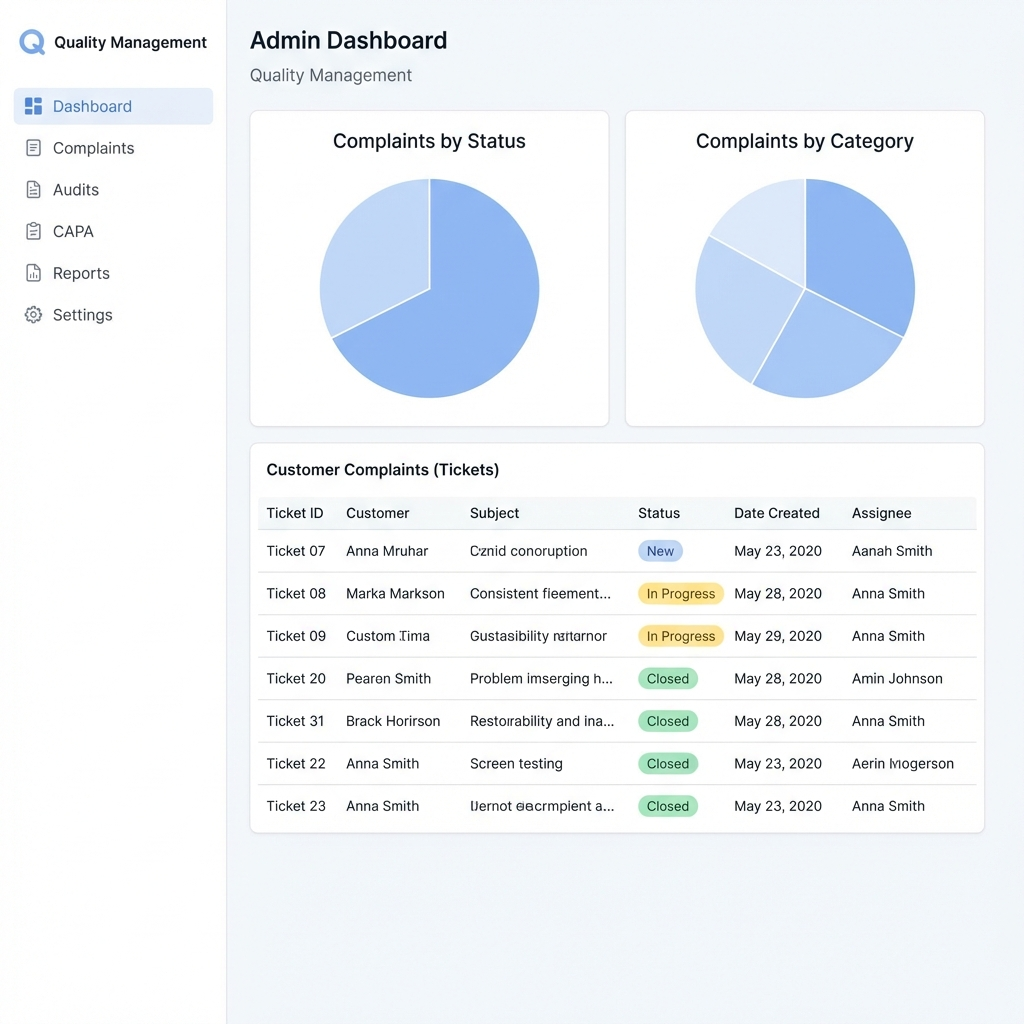
\includegraphics[width=14cm]{images/dashboard_rmq.png}
    \caption{Tableau de bord de gestion des réclamations -- Espace RMQ}
    \label{fig:dashboard-rmq}
\end{figure}

\subsubsection{Détail d'un Ticket}
Cette interface présente l'ensemble des informations d'une réclamation avec les actions disponibles (validation, refus, assignation fournisseur, changement de statut).

\begin{figure}[H]
    \centering
    \fbox{\parbox{12cm}{\centering\vspace{3cm}\textit{Capture d'écran à insérer}\\[0.5cm]\texttt{images/detail_ticket_rmq.png}\vspace{3cm}}}
    \caption{Interface de détail d'un ticket -- Espace RMQ}
    \label{fig:detail-rmq}
\end{figure}

\subsubsection{Module Statistiques}
Le module statistiques offre des graphiques et tableaux de bord analytiques pour le suivi des performances.

\begin{figure}[H]
    \centering
    \fbox{\parbox{12cm}{\centering\vspace{3cm}\textit{Capture d'écran à insérer}\\[0.5cm]\texttt{images/statistiques_rmq.png}\vspace{3cm}}}
    \caption{Module statistiques -- Espace RMQ}
    \label{fig:stats-rmq}
\end{figure}

% ==================================================
% ESPACE AQF
% ==================================================
\subsection{Espace Assistant Qualité Fournisseur (AQF)}

\subsubsection{Tableau de Bord AQF}
L'interface AQF affiche uniquement les tickets ayant un fournisseur assigné, permettant un suivi ciblé des réclamations liées aux fournisseurs.

\begin{figure}[H]
    \centering
    \fbox{\parbox{12cm}{\centering\vspace{3cm}\textit{Capture d'écran à insérer}\\[0.5cm]\texttt{images/dashboard_aqf.png}\vspace{3cm}}}
    \caption{Tableau de bord de l'espace AQF}
    \label{fig:dashboard-aqf}
\end{figure}

% ==================================================
% ESPACE ADMIN
% ==================================================
\subsection{Espace Administrateur}

\subsubsection{Gestion des Utilisateurs}
L'interface d'administration permet la gestion complète des utilisateurs du système (création, modification, activation/désactivation).

\begin{figure}[H]
    \centering
    \fbox{\parbox{12cm}{\centering\vspace{3cm}\textit{Capture d'écran à insérer}\\[0.5cm]\texttt{images/gestion_users_admin.png}\vspace{3cm}}}
    \caption{Interface de gestion des utilisateurs -- Espace Admin}
    \label{fig:admin-users}
\end{figure}

% ==================================================
% TESTS
% ==================================================
\section{Scénarios de Test}
Nous avons validé le fonctionnement via les tests fonctionnels suivants :

\begin{table}[H]
\centering
\begin{tabular}{|l|l|l|}
\hline
\textbf{Module} & \textbf{Action} & \textbf{Résultat Attendu} \\ \hline
Authentification & Saisir identifiants valides & Redirection vers Dashboard \\ \hline
Authentification & Saisir mot de passe incorrect & Message d'erreur affiché \\ \hline
Création Ticket & Envoyer formulaire vide & Blocage (Validation JS) \\ \hline
Création Ticket & Soumettre réclamation valide & Ticket créé + Email envoyé \\ \hline
Upload & Fichier invalide (.exe) & Rejet du fichier \\ \hline
Upload & Image valide (.jpg, .png) & Fichier enregistré \\ \hline
Validation RMQ & Valider un ticket & Statut mis à jour + Notification \\ \hline
Assignation & Assigner un fournisseur & Ticket visible dans AQF \\ \hline
\end{tabular}
\caption{Synthèse des tests fonctionnels réalisés}
\label{tab:tests}
\end{table}

\section{Sécurité}
Plusieurs mesures de sécurité ont été implémentées :
\begin{itemize}
    \item \textbf{Authentification :} Mots de passe hashés avec \texttt{password\_hash()}.
    \item \textbf{Sessions :} Gestion sécurisée des sessions PHP.
    \item \textbf{Requêtes préparées :} Utilisation de PDO pour prévenir les injections SQL.
    \item \textbf{Validation :} Contrôle des entrées utilisateur côté client et serveur.
    \item \textbf{Upload :} Restriction des types de fichiers autorisés.
\end{itemize}

\section*{Conclusion}
La phase de réalisation a permis de transformer les spécifications fonctionnelles et techniques en une application concrète et utilisable. L'architecture MVC et le choix des technologies ont facilité le développement d'une solution modulaire et évolutive. Les tests effectués confirment que le système est robuste et répond aux attentes initiales de la société SCPC Comptoir Hammami.

\newpage

\chapter*{Conclusion}
\addcontentsline{toc}{chapter}{Conclusion}

Ce stage de perfectionnement effectué au sein de la société \textbf{SCPC Comptoir Hammami} a été une expérience professionnelle et humaine d'une grande richesse. Il m'a offert l'opportunité de m'immerger dans le monde de l'entreprise et de comprendre les enjeux liés à la digitalisation des processus métiers.

\section*{Bilan du travail effectué}
L'objectif principal de ce stage était la conception et le développement de l'application "Central de Réclamation". Je peux affirmer que cet objectif a été atteint. L'application développée permet aujourd'hui :
\begin{itemize}
    \item Aux clients de saisir leurs réclamations en ligne de manière autonome.
    \item Au service qualité de centraliser toutes les demandes sur une plateforme unique.
    \item De suivre l'état d'avancement de chaque dossier en temps réel.
    \item De sécuriser les données qui étaient auparavant dispersées sur des supports papier ou Excel.
\end{itemize}

\section*{Apports du stage}
Sur le plan personnel et technique, ce stage m'a permis de :
\begin{itemize}
    \item \textbf{Consolider mes compétences techniques :} J'ai pu approfondir ma maîtrise du langage PHP et de la conception de bases de données relationnelles MySQL. J'ai également appris à structurer mon code selon une architecture MVC pour le rendre maintenable.
    \item \textbf{Découvrir le travail en équipe :} La collaboration avec le Responsable IT et les échanges avec le service Qualité m'ont appris l'importance de la communication et de l'écoute active pour bien cerner les besoins.
    \item \textbf{Gérer un projet :} J'ai appris à respecter un planning, à prioriser les tâches et à faire face aux imprévus techniques.
\end{itemize}

\section*{Perspectives d'amélioration}
Bien que fonctionnelle, l'application pourrait être enrichie par de nouvelles fonctionnalités :
\begin{itemize}
    \item \textbf{Module de statistiques avancé :} Génération automatique de graphiques (Camemberts, Histogrammes) pour analyser les types de défauts les plus fréquents.
    \item \textbf{Application Mobile :} Développement d'une version mobile native (Android/iOS) pour permettre aux clients d'envoyer des photos directement depuis leur smartphone sur le chantier.
    \item \textbf{Chatbot :} Intégration d'un assistant virtuel pour répondre aux questions fréquentes des clients avant qu'ils ne créent un ticket.
\end{itemize}

Pour conclure, cette expérience confirme ma volonté de poursuivre mes études dans le domaine du développement web et de l'ingénierie logicielle, afin de relever des défis encore plus complexes à l'avenir.

\newpage

\chapter*{Bibliographie et Nétographie}
\addcontentsline{toc}{chapter}{Bibliographie et Nétographie}

\section*{Ouvrages et Articles}
\begin{itemize}
    \item [1] Roques P., `UML2 par la pratique', Eyrolles 5ème édition, Aout 2006.
    \item [2] Nixon R., `Learning PHP, MySQL & JavaScript', O'Reilly Media, 2018.
\end{itemize}

\section*{Nétographie}
\begin{itemize}
    \item PHP Documentation. \url{https://www.php.net/docs.php} (Consulté le 15/01/2026)
    \item MySQL Reference Manual. \url{https://dev.mysql.com/doc/} (Consulté le 18/01/2026)
    \item W3Schools Online Web Tutorials. \url{https://www.w3schools.com} (Consulté le 20/01/2026)
    \item Stack Overflow. \url{https://stackoverflow.com} (Consulté régulièrement)
\end{itemize}

\newpage

\chapter*{Annexe}
\addcontentsline{toc}{chapter}{Annexe}

\section*{Annexe 1 : Modèle Relationnel de Données}
Le stockage des informations repose sur un modèle relationnel standard. Les principales tables sont les suivantes :

\begin{itemize}
    \item \textbf{Tickets} : Cette table centrale stocke toutes les réclamations, avec leur sujet, leur description, et les clés étrangères vers le client et le statut.
    \item \textbf{Utilisateurs} : Contient les informations de connexion (email, mot de passe haché) et les profils (Client, RMQ, Admin).
    \item \textbf{Statuts} : Définit le cycle de vie d'un ticket (Nouveau -> En cours -> Clôturé).
    \item \textbf{Historique} : Permet une traçabilité complète de chaque action effectuée sur un ticket (Qui a fait quoi et quand).
\end{itemize}


\end{document}
